\documentclass[12pt,a4paper]{article}
\usepackage{tabularx}
\usepackage{booktabs}
\usepackage{longtable}
\usepackage{ltxtable}
\usepackage[latin1]{inputenc}
\usepackage{amssymb}
\usepackage[]{graphicx,rotating}
\usepackage[T1]{fontenc}
\usepackage{parskip}
\usepackage{listings}
\usepackage{natbib}
\usepackage[official]{eurosym}
\usepackage{mathrsfs}
\usepackage{amsmath}
\usepackage{verbatim}
\usepackage{epstopdf} % to include eps files


\usepackage[usenames,dvipsnames]{color}     %for R colors and formatting
\usepackage{tikz,pgfplots,pgf}% for drawing neural net
\usepackage{neuralnetwork}
\usetikzlibrary{matrix,shapes,arrows,positioning}

\usepackage[left=3cm, right=2.5cm, top=2.5cm]{geometry}

\pagestyle{empty}
\parindent 0cm
\renewcommand{\baselinestretch}{1}
\newcommand{\bs}{\boldsymbol}
\renewcommand{\familydefault}{cmr} % alternative: cmss
\pdfminorversion=7
\bibliographystyle{agsm}
% for formatting packages, R, and Code
\newcommand{\pkg}[1]{{\normalfont\fontseries{b}\selectfont #1}}
\let\proglang=\textsf
\let\code=\texttt

\lstset{ %for R colors and formatting
  language=R,                     % the language of the code
  basicstyle=\scriptsize\ttfamily, % the size of the fonts that are used for the code
  numbers=left,                   % where to put the line-numbers
  numberstyle=\scriptsize\color{Blue},  % the style that is used for the line-numbers
  stepnumber=1,                   % the step between two line-numbers. If it is 1, each line
                                  % will be numbered
  numbersep=5pt,                  % how far the line-numbers are from the code
  backgroundcolor=\color{white},  % choose the background color. You must add \usepackage{color}
  showspaces=false,               % show spaces adding particular underscores
  showstringspaces=false,         % underline spaces within strings
  showtabs=false,                 % show tabs within strings adding particular underscores
  frame=single,                   % adds a frame around the code
  rulecolor=\color{black},        % if not set, the frame-color may be changed on line-breaks within not-black text (e.g. commens (green here))
  tabsize=2,                      % sets default tabsize to 2 spaces
  captionpos=b,                   % sets the caption-position to bottom
  breaklines=true,                % sets automatic line breaking
  breakatwhitespace=false,        % sets if automatic breaks should only happen at whitespace
  keywordstyle=\color{RoyalBlue},      % keyword style
  commentstyle=\color{YellowGreen},   % comment style
  stringstyle=\color{ForestGreen}      % string literal style
} 

\begin{document}

\begin{center}
% \vspace*{1cm}
 
\includegraphics[width=0.35\textwidth]{GU-Logo-blau-CMYK.eps} \vspace{2cm}
  
  {\Large{\bf Predicting Cross-Sell with Artificial Neural Networks}} \newline
  {\Large{An Empirical Study of ING's Customer Data}} \vspace{0.5cm}

  Seminar Thesis \\\vspace{2cm}
  submitted to \\\vspace{0.5cm}
  \textbf{Hon.-Prof. Dr. Martin Schmidberger} \\
  \textbf{Gabriela Alves Werb} \\\vspace{0.5cm}
  Goethe University Frankfurt am Main \\
  School of Business and Economics \\
  Chair for E-Commerce \vspace{2cm}
  
  by \\\vspace{0.5cm}
  \textbf{Lukas J\"urgensmeier} \\
  (Mat.-Nr.: 6904281) \\
  
  \medskip
  \medskip
  in partial fulfillment of the requirements \\
  for the degree of \\\vspace{0.5cm}
  \textbf{Master of Science in Business Administration} \\\vspace{0.5cm}
  July 31, 2019
  
\end{center}


\pagebreak
\pagestyle{plain}
\pagenumbering{Roman}
\tableofcontents
\listoffigures
\listoftables
\newpage
\setcounter{page}{2}
\pagenumbering{arabic}
\setlength{\baselineskip}{1.5\baselineskip}
\pagestyle{plain}


\section{Introduction}
\citep{hastieElementsStatisticalLearning2017}
Include research question here \\
\pkg{dplyr}
\proglang{R}
\code{a <- mutate(data, abc)}
Identify  addtitional  sales  potential in the client base to increase customer value and loyalty. \newline
Question: Will a customer buy an additional product? (yes/no) \newline
Goal: identify characteristics of typical customers who open a checking account and predict which customers
are likely open a checking account in the future
\section{Theoretical Background on Cross-sell}

\section{Methodology}
This section provides an overview over the implemented methodology by first outlining the feature engineering process that transforms the original data set
as required by neural networks.
The second part then describes the artificial neural network and its initial architecture, while the third part describes the hyperparameter tuning process
that leads to the \textit{best} model\footnote{This model is definitely not the best model \textit{existing}, but the best model \textit{found} through the trial-and-error tuning process.}.
Lastly, this section addresses a common criticism of machine learning technologies in general and neural networks in particular---the 
uninterpretable black box---by introducing the Local Interpretable Model-agnostic Explanation (LIME) as a method to 
"look under the hood" of a neural network and determine which features contributed by how much to a prediction.

\subsection{Feature Engineering and Data Set Preparation}
In order to feed seamlessly into a neural network, extensive feature engineering and data preparation is required \citep{hastieElementsStatisticalLearning2017}.
Before training the model, I (a) replace missing values in \code{pref\_device} and \code{occupation} by \code{None\_or\_missing},
(b) transform all \code{char} variables to a \code{factor} type, and (c) remove the misleading feature \code{ID}.
However, there are still numerous features including missing values. Since they are not missing at random, they need to be dealt with in order to not
bias the prediction.
Deleting all observations with missing values would do exactly that.
Hence, I impute missing values with a Random Forest from the \code{randomForest::rfImpute()} function.
This algorithm first replaces missing numeric (factor) variables with the median (mode) and then uses proximity measures from \code{randomForest}
as weights to replace \code{NA's} with the weighted average (the value with the highest proximity) of the non-missing values and repeats this for a
pre-defined number of iterations\footnote{After four iterations the out-of-bag error did not decrease visibly anymore, hence four iterations were chosen}
 \citep{liawClassificationRegressionRandomForest2002}.
I furthermore bin the continuous features \code{age}, \code{entry\_age} and \code{last\_acc}\footnote{Those two features exhibit a highly non-linear relationship.
According to the universal approximation theorem, a 
neural network with enough units in a hidden layer can approximate any continuous function \citep{hornikApproximationCapabilitiesMultilayer1991}.
Since the best neural network will be found by trying out different hyperparameters, including some which would not be "enough" hidden layer units, I bin
those two variables to make sure that this non-linear relationship can be taken into account by the model in any case. Also, the benchmark logit model
could not capture this effect without further specification.}.
Since a neural network cannot handle multi-categorical features, the routine dummy-codes those.
Finally---to not distort the input weights for the first hidden layer and thus not negatively affect the prediction quality 
\citep[pp. 398]{hastieElementsStatisticalLearning2017}---I center and scale all input features to exhibit $\bar{x}=0$ and $s=1$.
The feature engineered data set consists of $N=72$ input variables that will be used to predict cross-sell. 
\begin{figure}[ht]
	\centering
  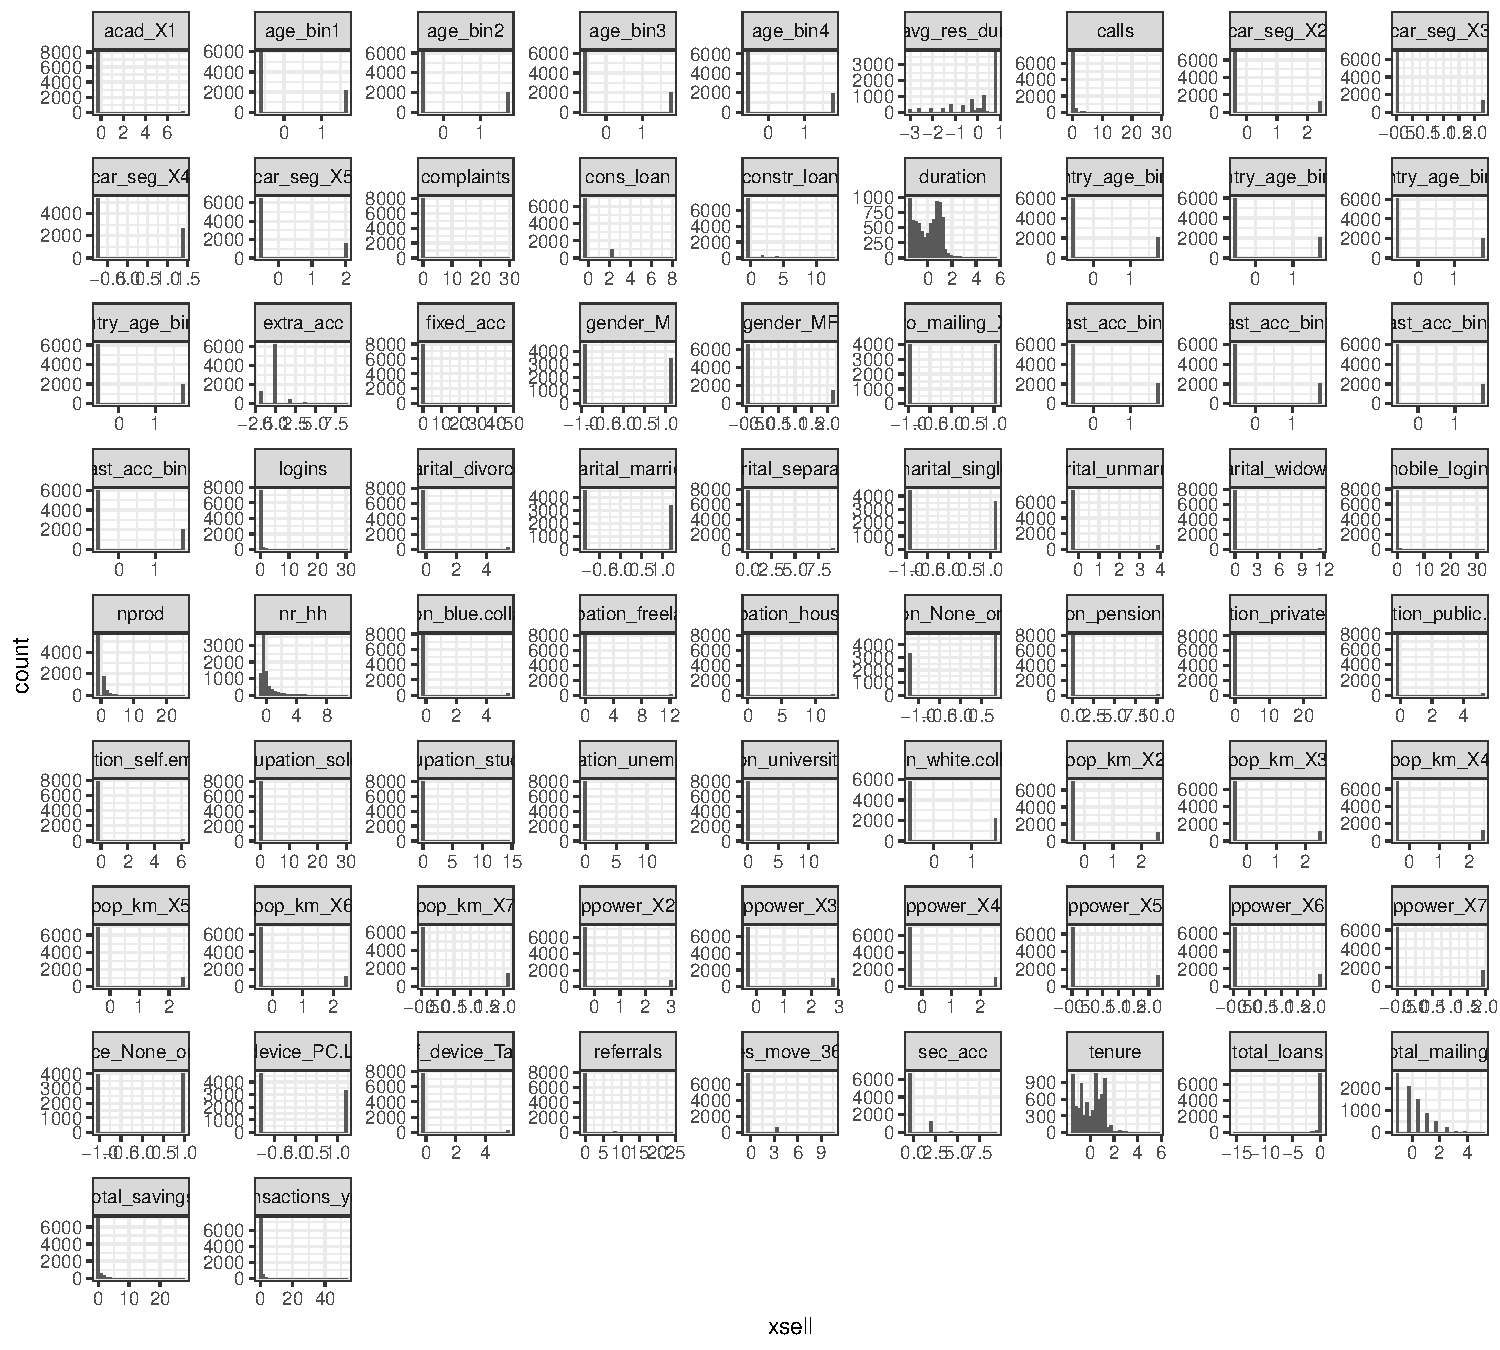
\includegraphics[scale=0.63]{figures/hist_all_features.pdf}
	\caption{Histogram of all features after feature engineering process}
	\label{fig_hist}
\end{figure}Figure \ref{fig_hist} displays the histograms for each
of those features.




\begin{figure}[ht]
	\centering
  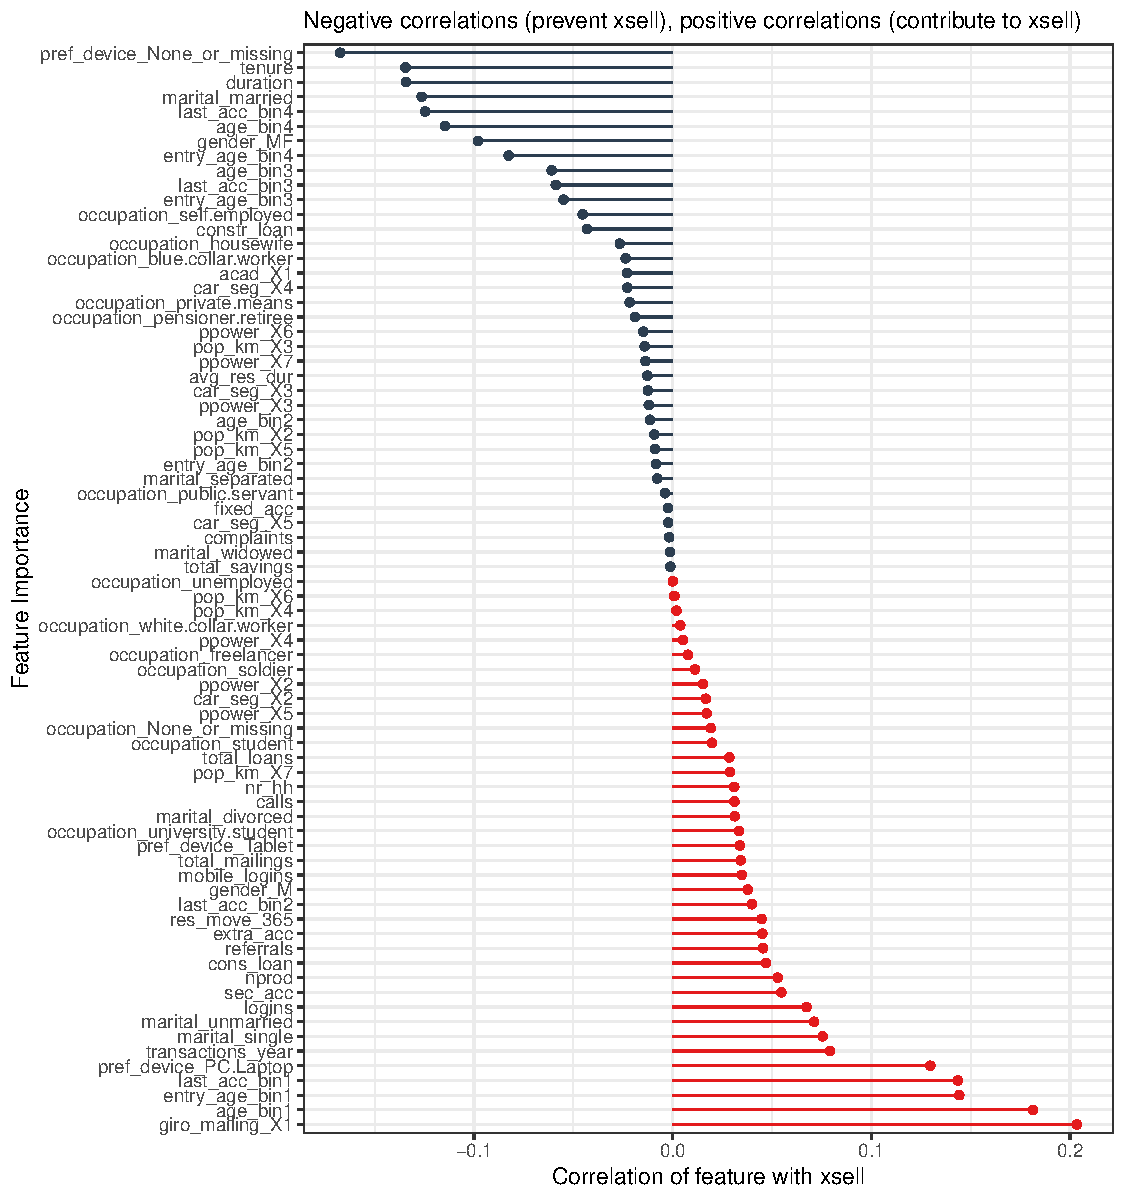
\includegraphics[scale=0.8]{figures/corrplot.pdf}
	\caption{Correlation of feature engineered variables with xsell}
	\label{fig_corr}
\end{figure}

\subsection{Artificial Neural Network with Keras}
\subsection{Hyperparameter Tuning}


\begin{figure}
\begin{center}
\def\layersep{3.5cm}

\begin{tikzpicture}[
   shorten >=1pt,->,
   draw=black!50,
    node distance=\layersep,
    every pin edge/.style={<-,shorten <=1pt},
    neuron/.style={circle,fill=black!25,minimum size=17pt,inner sep=0pt},
    input neuron/.style={neuron, fill=green!50},
    output neuron/.style={neuron, fill=red!50},
    hidden neuron/.style={neuron, fill=blue!50},
    annot/.style={text width=4em, text centered}
]

    % Draw the input layer nodes
    \foreach \name  [count=\y] in 
    {acad\_X1, age\_bin1, \dots,  age\_bin4, mobile\_logins, tenure, \dots, total\_mailings, transactions\_year}
     {   \node[input neuron, pin=left:\name] (I-\y) at (0,-\y cm) {};  
     }

    % set number of hidden layers
    \newcommand\Nhidden{2}
    \newcommand\NodOne{5}
    \newcommand\NodTwo{10}
    \newcommand\Nod{9}

    % Draw the hidden layer nodes
%    \foreach \N in {1,...,\Nhidden} {

     \foreach \y in {1,...,\NodOne} {
          \path[yshift=-1.80cm]
              node[hidden neuron] (H1-\y) at (1*\layersep,-\y cm) {};
              }
    \node[annot,above of=H1-1, node distance=2.8cm] (hl1) {Hidden layer 1};
     \foreach \y in {1,...,\NodTwo} {
          \path[yshift=0cm]
              node[hidden neuron] (H2-\y) at (2*\layersep,-\y cm) {};            
           }
    \node[annot,above of=H2-1, node distance=1cm] (hl2) {Hidden layer 2};          

%    }

    \node[below=3.2cm of H1-\NodOne] (text1) {64 neurons};
    \node at (text1 -| H2-1) (text2) {128 neurons};
	\node at (text1 -| I-9) (text1) {74 inputs};

    % Draw the output layer node
    \node[output neuron,pin={[pin edge={->}]right:xsell}, right of=H\Nhidden-5] (O) {};

    \node at (text1 -| O) (text3) {1 output};
    % Connect every node in the input layer with every node in the
    % hidden layer.
    \foreach \source in {1,...,9}{
        \foreach \dest in {1,...,\NodOne}{
            \path (I-\source) edge (H1-\dest);
         }
    }
    % connect all hidden stuff
    \foreach [remember=\N as \lastN (initially 1)] \N in {2,...,\Nhidden}
       \foreach \source in {1,...,\NodOne}
           \foreach \dest in {1,...,\NodTwo}
               \path (H\lastN-\source) edge (H\N-\dest);

    % Connect every node in the hidden layer with the output layer
    \foreach \source in {1,...,\NodTwo}
        \path (H\Nhidden-\source) edge (O);

    % Annotate the layers

    \node[annot,left of=hl1] {Input layer};
    \node[annot,right of=hl\Nhidden] {Output layer};
\end{tikzpicture}
% End of code
\label{fig_nn_arch}
\caption{Architecture of the Artificial Neural Network implemented in this study}
\end{center}
\end{figure}

\begin{figure}[ht]
	\centering
  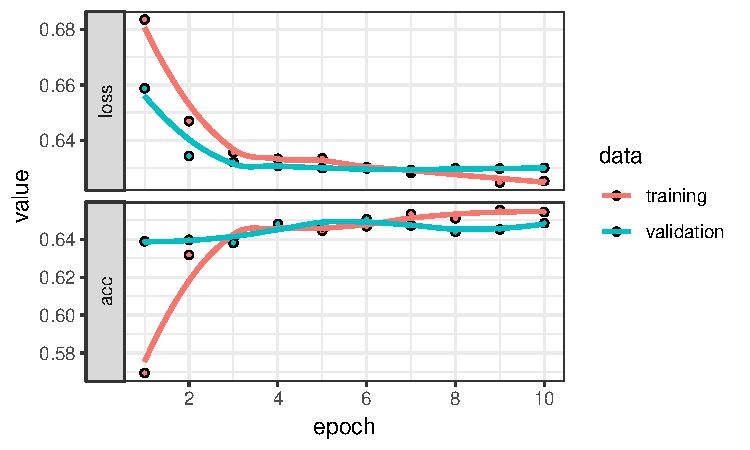
\includegraphics[scale=0.8]{figures/train_history.pdf}
	\caption{Loss and accuracy for training and test data over training history of the tuned model}
	\label{fig_history}
\end{figure}

\subsection{Local Interpretable Model-agnostic Explanation (LIME)}
\section{Results and Model Comparison}
\subsection{Comparing the Predicions of ANN with the Benchmark Logit Model}

\begin{figure}[ht]
	\centering
  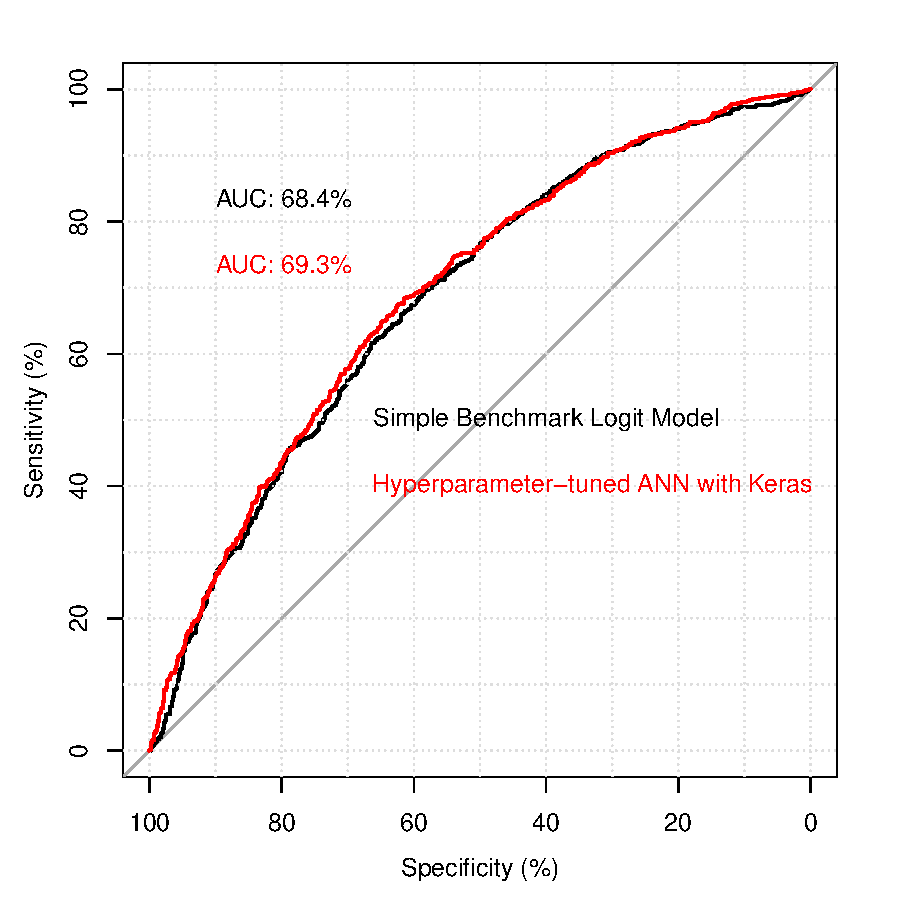
\includegraphics[scale=0.63]{figures/roc_auc_comp.pdf}
	\caption{ROC curve comparison between benchmark logit and hyperparameter-tuned neural network predictions}
	\label{fig_roc}
\end{figure}


%Comparison of Model Statistics
\begin{table}[!htbp] \centering
\caption{Model performance comparison---statistics and confusion matrix}
\label{tab_comparemodel} 
{\small
\begin{tabular}{@{\extracolsep{5pt}} ccccccccc} 
\\[-1.8ex]\hline 
\hline \\[-1.8ex] 
\multicolumn{3}{c}{\textit{Benchmark Logit}} & \multicolumn{3}{c}{\textit{Hyperparameter-tuned ANN}} \\ \hline
Accuracy & 0.6463 &  & Accuracy & 0.6423 &  \\
Sensitivity & 0.6653 &  & Sensitivity & 0.7331 &  \\
Specificity & 0.6271 &  & Specificity & 0.5508 &  \\
Pos Pred Value & 0.6429 &  & Pos Pred Value & 0.6221 &  \\
Neg Pred Value & 0.6500 &  & Neg Pred Value & 0.6716 &  \\
Kappa & 0.2925 &  & Kappa & 0.2841 &  \\
Prevalence & 0.5023 &  & Prevalence & 0.5023 &  \\
\hline \\[-1.8ex] 
 & \multicolumn{2}{c}{\textit{Actual}} &  & \multicolumn{2}{c}{\textit{Actual}} \\
\multicolumn{1}{r}{\textit{Prediction}} & 0 & \multicolumn{1}{c}{1} & \multicolumn{1}{r}{\textit{Prediction}} & 0 & \multicolumn{1}{c}{1} \\ 
\multicolumn{1}{r}{0} & 624 & \multicolumn{1}{c}{336} & \multicolumn{1}{r}{0} & 548 & \multicolumn{1}{c}{268} \\
\multicolumn{1}{r}{1} & 371 & \multicolumn{1}{c}{668} & \multicolumn{1}{r}{1} & 447 & \multicolumn{1}{c}{736} \\
\hline \\[-1.8ex] 
\end{tabular}
}
\end{table}

\begin{table}[!htbp] \centering 
  \caption{Resulting statistics of 324 hyperparameter tuning model runs} 
  \label{tab_hypertune} 
\begin{tabular}{@{\extracolsep{5pt}} ccccccccc} 
\\[-1.8ex]\hline 
\hline \\[-1.8ex] 
rank & val\_acc & acc & units1 & dropout1 & units2 & dropout2 & epochs &batch \\ 
\hline \\[-1.8ex] 
1 & $0.656$ & $0.654$ & $64$ & $0.600$ & $128$ & $0.600$ & $10$ & $100$ \\ 
2 & $0.654$ & $0.692$ & $128$ & $0.600$ & $64$ & $0.600$ & $30$ & $150$ \\ 
3 & $0.653$ & $0.674$ & $64$ & $0.600$ & $64$ & $0.600$ & $30$ & $100$ \\ 
4 & $0.651$ & $0.658$ & $64$ & $0.600$ & $64$ & $0.600$ & $10$ & $100$ \\ 
5 & $0.651$ & $0.673$ & $64$ & $0.600$ & $128$ & $0.600$ & $30$ & $50$ \\ 
$\dots$ & $\dots$ & $\dots$ & $\dots$ & $\dots$ & $\dots$ & $\dots$ & $\dots$ & \dots  \\
323 & $0.604$ & $0.731$ & $64$ & $0.200$ & $32$ & $0.400$ & $30$ & $128$ \\ 
324 & $0.602$ & $0.735$ & $64$ & $0.200$ & $32$ & $0.200$ & $30$ & $128$ \\ 
\hline \\[-1.8ex] 
\end{tabular} 
\end{table} 



\subsection{Beyond the Black Box: Feature Importance with LIME}

\begin{figure}[ht]
	\centering
  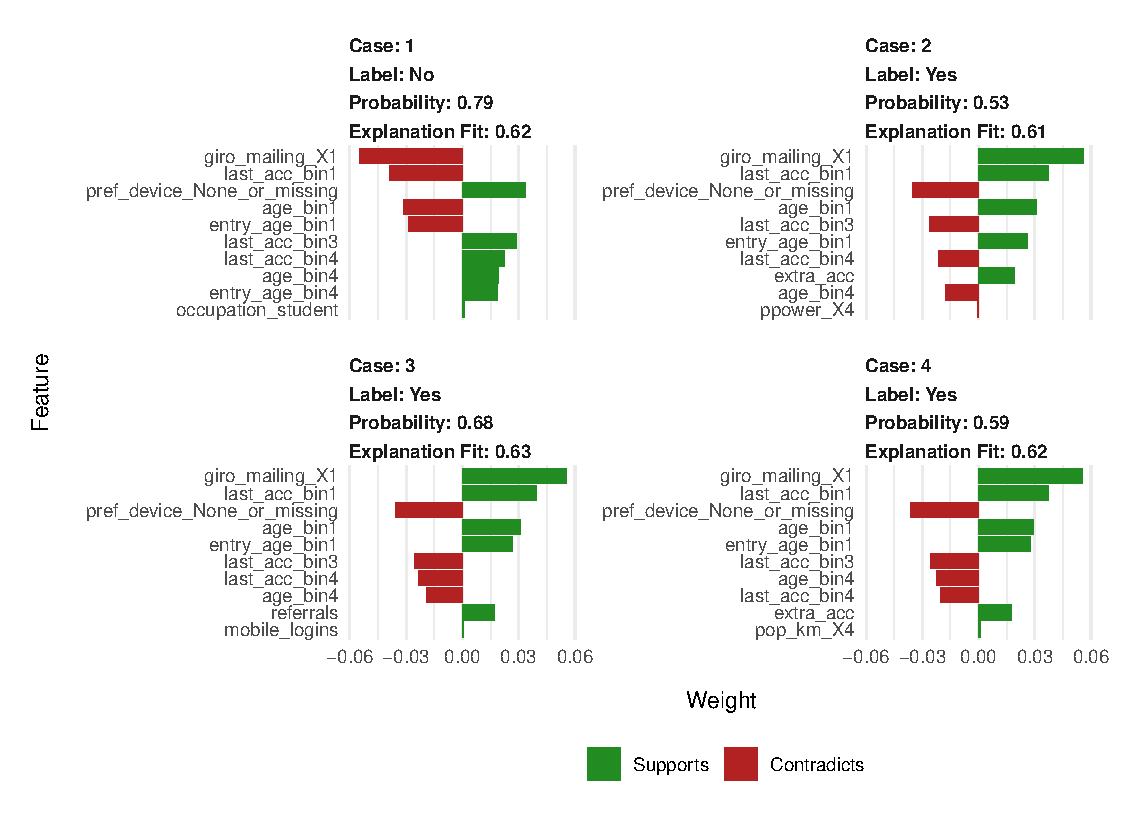
\includegraphics[scale=0.83]{figures/lime_first_four.pdf}
	\caption{LIME feature importance of the ten most important features for each of the first four customers in the test data set}
	\label{fig_lime_four}
\end{figure}

\begin{figure}[ht]
	\centering
  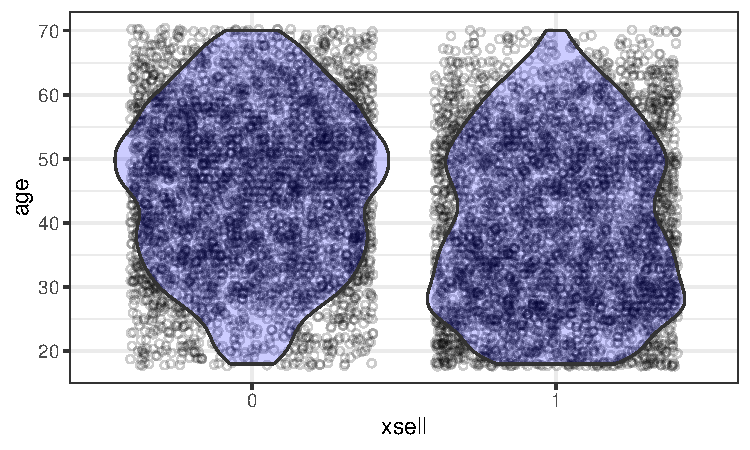
\includegraphics[scale=0.83]{figures/violin_age_xsell.pdf}
	\caption{Individual variable assessment---violin plot of xsell vs. age}
	\label{fig_lime_four}
\end{figure}




\section{Managerial and Research Implications}
\section{Conclusion}




\clearpage
\appendix
\section{R Code}

\clearpage
\bibliography{library}

\newpage
\thispagestyle{empty}
\section*{Statutory Declaration}\label{statutory-declaration}

I herewith declare that I have completed the present thesis independently, without making use of
other than the specified literature and aids. Sentences or parts of sentences quoted literally are
marked as quotations; identification of other references with regard to the statement and scope of
the work is quoted. The thesis in this form or in any other form has not been submitted to an examination body and has not been published.
This thesis has not been used, either in whole or part, for another examination achievement.

\vspace{1cm}

Frankfurt am Main, July 31, 2019
\vspace{2cm}

. . . . . . . . . . . . . . . . . . . . . . . . . . . . . . .
\vspace{0.1cm}

Lukas J\"urgensmeier
\end{document}
